\documentclass[
	a4paper,
	pagesize,
	pdftex,
	12pt,
	twoside, % + BCOR darunter: für doppelseitigen Druck aktivieren, sonst beide deaktivieren
	BCOR=5mm, % Dicke der Bindung berücksichtigen (Copyshop fragen, wie viel das ist)
	ngerman,
	fleqn,
	final,
	]{scrartcl}
\usepackage{ucs}
\usepackage[utf8x]{inputenc} % Eingabekodierung: UTF-8
\usepackage{fixltx2e} % Schickere Ausgabe
\usepackage[T1]{fontenc} % ordentliche Trennung
\usepackage[english]{babel}
\usepackage{lmodern} % ordentliche Schriften
\usepackage[unicode=true]{hyperref}
\usepackage{setspace,graphicx,tikz,tabularx} % für Elemente der Titelseite
\usepackage[draft=false,babel,tracking=true,kerning=true,spacing=true]{microtype} % optischer Randausgleich etc.

% figure stuff
\usepackage{caption}
\usepackage{subcaption}
\usepackage{wrapfig}

% no indent
\setlength\parindent{0pt}

% code snippet settings
\usepackage{listings}
\usepackage{color}

\definecolor{dkgreen}{rgb}{0,0.6,0}
\definecolor{gray}{rgb}{0.5,0.5,0.5}
\definecolor{mauve}{rgb}{0.58,0,0.82}

\lstset{
  frame=single,
  language=Java,
  aboveskip=3mm,
  belowskip=3mm,
  showstringspaces=false,
  columns=flexible,
  basicstyle={\small\ttfamily},
  numbers=none,
  numberstyle=\tiny\color{gray},
  keywordstyle=\color{blue},
  commentstyle=\color{dkgreen},
  stringstyle=\color{mauve},
  breaklines=true,
  breakatwhitespace=true,
  tabsize=2
}






\begin{document}

% Beispielhafte Nutzung der Vorlage für die Titelseite (bitte anpassen):
% LaTeX-Vorlage für die Titelseite und Selbständigkeitserklärung einer Abschlussarbeit
% basierend auf der vorigen Institutsvorlage des Instituts für Informatik
% sowie der Vorlage für Promotionsarbeiten.
%
% erweitert: 2014-06-12 Dennis Schneider <dschneid@informatik.hu-berlin.de>

% gepunktete Linie unter Objekt:
\newcommand{\TitelPunkte}[1]{%
  \tikz[baseline=(todotted.base)]{
    \node[inner sep=1pt,outer sep=0pt] (todotted) {#1};
    \draw[dotted] (todotted.south west) -- (todotted.south east);
  }%
}%

% gepunktete Linie mit gegebener Länge:
\newcommand{\TitelPunktLinie}[1]{\TitelPunkte{\makebox[#1][l]{}}}

\makeatletter

\newcommand*{\@titelTitel}{Titel der Arbeit}
\newcommand{\titel}[1]{\renewcommand*{\@titelTitel}{#1}} % Titel der Arbeit
\newcommand*{\@titelArbeit}{Arbeitstyp}
\newcommand{\typ}[1]{\renewcommand*{\@titelArbeit}{#1}} % Typ der Arbeit
\newcommand*{\@titelGrad}{akademischer Grad}
\newcommand{\grad}[1]{\renewcommand*{\@titelGrad}{#1}} % Akademischer Grad
\newcommand*{\@titelAutor}{Autor}
\newcommand{\autor}[1]{\renewcommand*{\@titelAutor}{#1}} % Autor der Arbeit
\newcommand*{\@titelGeburtsdatum}{\TitelPunktLinie{2cm}}
\newcommand{\gebdatum}[1]{\renewcommand*{\@titelGeburtsdatum}{#1}} % Geburtsdatum des Autors
\newcommand*{\@titelGeburtsort}{\TitelPunktLinie{5cm}}
\newcommand{\gebort}[1]{\renewcommand*{\@titelGeburtsort}{#1}} % Geburtsort des Autors
\newcommand*{\@titelGutachterA}{\TitelPunktLinie{5cm}}
\newcommand*{\@titelGutachterB}{\TitelPunktLinie{5cm}}
\newcommand{\gutachter}[2]{\renewcommand*{\@titelGutachterA}{#1}\renewcommand*{\@titelGutachterB}{#2}} % Erst- und Zweitgutachter
\newcommand*{\@titelEinreichungsdatum}{\TitelPunktLinie{3cm}} % Datum der Einreichung, wird nicht vom Studenten ausgefüllt
\newcommand*{\@titelVerteidigungsdatum}{} % Verteidigungstext, wird nicht vom Studenten ausgefüllt
\newcommand{\mitverteidigung}{\renewcommand*{\@titelVerteidigungsdatum}{verteidigt am: \,\,\TitelPunktLinie{3cm}}} % Verteidigungsplatzhalter erzeugen
\newcommand*{\@wastwoside}{}

% Titelseite erzeugen:
\newcommand{\makeTitel}{%
	% Speichere, ob doppelseitiges Layout gewählt wurde:
\if@twoside%
	\renewcommand*{\@wastwoside}{twoside}
\else
	\renewcommand*{\@wastwoside}{twoside=false}
\fi
	\KOMAoptions{twoside = false}% Erzwinge einseitiges Layout (erzeugt eine Warnung)

	\begin{titlepage}
		% Ändern der Einrückungen
		\newlength{\parindentbak} \setlength{\parindentbak}{\parindent}
		\newlength{\parskipbak} \setlength{\parskipbak}{\parskip}
		\setlength{\parindent}{0pt}
		\setlength{\parskip}{\baselineskip}

		\thispagestyle{empty}

		\begin{minipage}[c][3cm][c]{12cm}
			\textsc{%
				% optischer Randausgleich per Hand:
				\hspace{-0.4mm}\textls*[68]{\Large Humboldt-Universität zu Berlin}\\
				\normalsize \textls*[45]{
					Mathematisch-Naturwissenschaftliche Fakultät\\
					Institut für Informatik
				}
			}
		\end{minipage}
		\hfill
		\begin{minipage}[c][3cm][c]{3cm}
			
\includegraphics[width=3cm]{husiegel.pdf}
		\end{minipage}

		% Also wenn schon serifenlose Schriften (Titel), dann ganz oder gar nicht
		\sffamily

		\vfill

		\begin{center}
		\begin{doublespace}
			\vspace{\baselineskip}
			{\LARGE \textbf{\@titelTitel}}\\
			%\vspace{1\baselineskip}
			{\Large
				\@titelArbeit\\
				zur Erlangung des akademischen Grades\\
				\@titelGrad
				\vspace{\baselineskip}
			}
		\end{doublespace}
		\end{center}

		\vfill
\newcolumntype{L}{>{\raggedright\arraybackslash}X}
		{\large \raggedleft
			\begin{tabularx}{\textwidth}{l@{\,\,\raggedright~}L} % verbreiterter Abstand zwischen Feldern wurde gewünscht
				eingereicht von: & \@titelAutor\\
				geboren am: & {\@titelGeburtsdatum}\\
				geboren in: & \@titelGeburtsort
				\vspace{0.5\baselineskip}\\
				Gutachter/innen: & \@titelGutachterA \\
					& \@titelGutachterB
				\vspace{0.5\baselineskip}\\
				eingereicht am: & \@titelEinreichungsdatum \hfill \@titelVerteidigungsdatum
			\end{tabularx}}
			\vspace{-1\baselineskip}\\\phantom{x} % Übler Hack, um eine Warnung wg. einer zu leeren hbox zu verhindern
		% Wiederherstellen der Einrückung
		\setlength{\parindent}{\parindentbak}
		\setlength{\parskip}{\parskipbak}
	\end{titlepage}

	% Aufräumen:
	\let\@titelTitel\undefined
	\let\titel\undefined
	\let\@titelArbeit\undefined
	\let\typ\undefined
	\let\@titelGrad\undefined
	\let\grad\undefined
	\let\@titelAutor\undefined
	\let\autor\undefined
	\let\@titelGeburtsdatum\undefined
	\let\gebdatum\undefined
	\let\@titelGeburtsort\undefined
	\let\gebort\undefined
	\let\@titelGutachterA\undefined
	\let\@titelGutachterB\undefined
	\let\gutachter\undefined
	\let\@titelEinreichungsdatum\undefined
	\let\einreichungsdatum\undefined
	\let\@titelVerteidigungsdatum\undefined
	\let\verteidigungsdatum\undefined

	\KOMAoptions{\@wastwoside}% Stelle alten Modus (ein-/doppelseitig) wieder her
	\let\@wastwoside\undefined
	\cleardoublepage % ganzes Blatt für die Titelseite
}

% Als Allerallerletztes kommt Selbständigkeitserklärung:
% Aufruf mit dem Datum in deutscher und englischer Form
\newcommand{\selbstaendigkeitserklaerung}[1]{%
	\cleardoublepage% Wieder auf eine eigene Doppelseite
	{\parindent0cm
		\subsection*{Selbständigkeitserklärung}
		Ich erkläre hiermit, dass ich die vorliegende Arbeit selbständig verfasst
		und noch nicht für andere Prüfungen eingereicht habe.
		Sämtliche Quellen einschließlich Internetquellen, die unverändert oder
		abgewandelt wiedergegeben werden, insbesondere Quellen für Texte, Grafiken,
		Tabellen und Bilder, sind als solche kenntlich gemacht. Mir ist bekannt,
		dass bei Verstößen gegen diese Grundsätze ein Verfahren wegen
		Täuschungsversuchs bzw. Täuschung eingeleitet wird.
		\vspace{3\baselineskip}

		{\raggedright Berlin, den #1 \hfill \TitelPunktLinie{8cm}\\}
% Bitte verwenden Sie diese Erklaerung auch fuer englischsprachige Arbeiten. Eine Uebersetzung ist nicht zweckmaessig.
	}
}%

\makeatother



\titel{Drift: an imperative programming environment for the cloud} % Titel der Arbeit
\typ{Masterarbeit} % Typ der Arbeit:  Diplomarbeit, Masterarbeit, Bachelorarbeit
\grad{Master of Science (M. Sc.)} % erreichter Akademischer Grad
% z.B.: Master of Science (M. Sc.), Master of Education (M. Ed.), Bachelor of Science (B. Sc.), Bachelor of Arts (B. A.), Diplominformatikerin
\autor{Frank Lange} % Autor der Arbeit, mit Vor- und Nachname
\gebdatum{08.08.1989} % Geburtsdatum des Autors
\gebort{Berlin} % Geburtsort des Autors
\gutachter{Prof. Dr. Jens-Peter Redlich}{Prof. Dr. Joachim Fischer} % Erst- und Zweitgutachter der Arbeit
\mitverteidigung % entfernen, falls keine Verteidigung erfolgt
\makeTitel

% Hier folgt die eigentliche Arbeit (bei doppelseitigem Druck auf einem neuen Blatt):
\tableofcontents
\thispagestyle{empty}


\newpage
\thispagestyle{empty}
\ \\

\newpage
\thispagestyle{empty}

\vspace*{\fill}
\begin{quote}
\centering
\textit{``If I had more time, I would have written a shorter letter.''}
\\
\ \\
-- Blaise Pascal
\end{quote}
\vspace*{\fill}

\newpage
\thispagestyle{empty}
\ \\

\newpage

\section{Introduction}
Alongside the advent of multi-core CPU architectures
and increased local storage capacities, large scale distributed
systems based on commodity hardware, accommondated for in special
facilities like data centers, have proven to be a viable tool for
dealing with the ever increasing demand of compute power and
storage.

One of the largest drivers of this demand is of course
the modern web, including not only all the data accumulation
that is taking place on social networks and social media but also
providing different kinds of large scale services and platforms
like maps and navigations but also e-commerce platforms which
today include music and video streaming platforms like
\textit{Spotify}, \textit{Netflix} or \textit{Amazon Prime Music} or
\textit{Amazon Prime Video} or even transportation-on-demand
platforms like \textit{Uber}.

Additionally, the advent of artificial intelligence and
machine learning created its own demand for ever increasing
large scale neural networks and training data sets. A progression
that is deeply coupled with the products of the modern web,
providing not only recommondation or prediction engines for
the users but also scheduling and load balancing decisions
inside the systems, perfectly adapted to the given workload,
which allow to fully utilize a given system to capacity without
human intervention.
\newline

Therefore, in order to provide systems that allow to scale to millions
or even billions of users, either in terms of storage, computing,
training neural networks or simply content delivery and response times,
large scale distributed systems have been constructed which pose new
system design challenges not only regarding fault tolerance, network failure
and fail over strategies but also in terms of simply how to
describe, express and comprehend these vast and infinitely
complex systems.








\subsection{Goal of this work}
To face these challenges and to analyze and explore the
concepts needed by software engineers to describe, construct and program
these system, the following work presents the
\textit{Drift Programming Environment}, a collection of different
components that allow the programming and orchestration of a
distributed system of autonomous services by describing
their data dependencies.

The goal of this work is to not only present each individual
component of the final result, which includes an abstract,
imperative and stateful coordination language, an immutable
file system based on distributed message queues and an interactive
user interface based on the syntax of Petri Nets,
but also to introduce the reader to the set of projects and the
people that created these projects, and their ideas and philosophies,
that served as inspirations and guidance for the ideas and design decisions
included in the \textit{Drift} project.





\subsection{Structure of this work}
This is done by giving a short summary of the history and
evolution of programming languages and their adaption to
fundamental changes of the underlying hardware, especially the
advent of distributed systems in chapter \ref{distributedprogramming}.

Chapter \ref{relatedwork} then succesively introduces the related
projects and tries to extract and hightlight their relevant aspects
to the \textit{Drift} project.

Chapter \ref{drift} then introduces the components of the
\textit{Drift Programming Environment} by first introducing the
Drift language in chapter \ref{driftlang} including its implementation
in form the of the Drift shell. This is followed by the introduction
of the Drift system implementation in chapter
\ref{driftimplementation} including an extensive explanation of
the error model and distributed error handling procedure.
Finally, chapter \ref{driftui} presents the Drift UI prototype
which features the Drift shell as introduced in chapter \ref{driftshell}
as well as an interactive graphical representation of the
current state of the entire system using the Petri Net syntax
and an event time line that allows to effortlessly review previews
system states.

Chapter \ref{summary} then summarizes the presented work, including
all the presented components and their contribution to the overall
system and chapter \ref{futurework} thoroughly discusses possible
improvements regarding the implementation of each individual component
as it was introduced in chapter \ref{drift} as well as possible
progressions of future projects.

\section{Distributed Programming}
In 1937 a paper titled \textit{``On computable numbers, with an
application to the Entscheidungsproblem''}, written by Alan Turing, was
published \cite{turingcomputable}. In it Turing defines what is now
known as a \textit{Turing machine}, a theoretical machine model for
executing arbitrary computation. He demonstrates how to formulate
instructions for this machine in order to configure its execution
behavior and goes so far as to show how this
machine could even receive another machine configuration as its input
and then execute what the other machine would have done, thereby
effectively emulating the given machine.
\newline

But he wasn't the only one thinking about computation. As summarized
by Denning in \cite{whatiscomputation}, Kurt Gödel, Alonzo Church and Emil
Post all contributed to the task of exploring the boundaries of
computation, setting the tone for the next 80 years of research
concerning \textit{computation}, \textit{computers} and \textit{automation}.

Of all the proposed approaches of how to tackle the concept of computation
and turning it into a tool that could be understood and used by delivering
a theoretical framework, one could argue that Turing's machine model
emerged as a winner because, although not at the time, it turned out
to be closest to what machines became to be. How they were structed and
how they basically operated. Still, to this day.

So in order to use or \textit{program} these machines, these computers,
programming languages were developed and over the decades have gone
through their own evolutionary process \cite{pl-gens} with the
first generation using binary machine instructions to todays languages
that allow for higher level programming styles like
\textit{object oriented programming } \cite{bjarneOO} or
\textit{functional programming} \cite{wadler-functional}.
\newline

But no matter what mainstream programming language one looks at today,
they all seem to have one thing in common, which also gets replicated
by each new language that arrives: they are all focussing on
describing computation. Computation executed by a single core machine.
Because for most of the last century, this was the problem we were
facing.

However, with the advent of commodity multicore hardware
\cite{core2duo} the problem domain changed. Now a machine isn't
a single machine anymore, but rather a group of multiple CPU cores
that can operate and compute independent of each other.

Unfortunately mainstream languages are still struggling with delivering
language concepts and semantics that allow for utilizing this new
hardware. In Fig.\ref{pythreads} one can see a very minimal multithreaded
program written in Python, one of the most used languages today
\cite{langrank}.


\begin{wrapfigure}{l}{0.55\textwidth}
  \vspace{-10pt}
  \begin{center}
    \begin{lstlisting}
from threading import Thread

def count(n):
  while n > 0:
    n -= 1

t1 = Thread(target=count,args=(1000000,))
t1.start()

t2 = Thread(target=count,args=(1000000,))
t2.start()

t1.join()
t2.join()
    \end{lstlisting}
  \end{center}
  \vspace{-20pt}
  \caption{Python multithreading example}
  \label{pythreads}
\end{wrapfigure}

As was shown by Beazley in \cite{pygil} this multithreaded version is up to
\textit{two times} slower than the single threaded version and the
reason for this is the so called \textit{Global Interpreter Lock}
(GIL) used by the Python interpreter which basically prevents multiple
native threads from truly executing in parallel.

This shows how important it is to reevaluate exisiting programming
languages and methodologies whenever the underlying machine or system
changes dramatically.
\newline

Another such paradigm shift was the advent of
the \textit{internet}, or large scale networking in general, because it
dawned what is now known as the \textit{information age}. Although this
is a rather broad term, describing global change in almost all areas of
modern civilization, I believe these changes can also be seen in the area
of computing and computation. Because in order to deliver products
like: the world wide web, internet search, internet advertising,
social networks, social media, music streaming,
video streaming, messenger services, navigation/maps, e-commerce etc.
companies had to build massive computer networks in order to either store
massive amounts of data or to simply scale their
product to millions or billions of users.
And altough almost all of the current products, apps, or services
could not exist, without the computation that is implemented inside
their core parts, it is \textit{communication} that has become the
main obstacle for building large scale \textit{information systems}.

\subsection{Language Evolution}
\label{LanguageEvolution}

But no matter what mainstream programming language one looks at today,
they all seem to have one thing in common, which also gets replicated
by each new language that arrives: they are all focussing on
describing computation. Computation executed by a single core machine.
Because for most of the last century, this was the problem we were
facing.

However, with the advent of commodity multicore hardware
\cite{core2duo} the problem domain changed. Today even a single a machine
isn't a single machine anymore, but rather a group of multiple CPU cores
that can operate and compute independent of each other.

Unfortunately mainstream languages are still struggling with delivering
language concepts and \textit{semantics} that allow for utilizing this new
hardware. In Fig.\ref{pythreads} one can see a very minimal multithreaded
program written in Python, one of the most used languages today
\cite{langrank}.


\begin{wrapfigure}{l}{0.55\textwidth}
    \begin{lstlisting}
from threading import Thread

def count(n):
  while n > 0:
    n -= 1

t1 = Thread(target=count,args=(1000000,))
t1.start()

t2 = Thread(target=count,args=(1000000,))
t2.start()

t1.join()
t2.join()
    \end{lstlisting}
  \caption{Python multithreading example}
  \label{pythreads}
\end{wrapfigure}

As was shown by Beazley in \cite{pygil} this multithreaded version is up to
two times \textit{slower} than the single threaded version and the
reason for this is the so called \textit{Global Interpreter Lock}
(GIL) used by the Python interpreter which basically prevents multiple
native threads from truly executing in parallel.

This is supposed to show how slow adoption and adjustment in the mainstream
programming language market is happening, even for a problem domain that,
as I would like to argue, is not even the most recent set of problems
programmers today need to deal with.

This shows how important it is to reevaluate exisiting programming
languages, their implementations and their methodologies whenever the
underlying machine, system or problem domain changes dramatically.
\newline

Now one could argue that Python might have been a bad example and
that other mainstream languages offer better adoption of
multithreaded programming. Fig \ref{thread-examples}
shows another two examples of how threading is expressed in programming today,
namely using the programming languages \textit{Java} \cite{java} and
\textit{Go} \cite{golang}. Altough Java and its virtual runtime environment, the
\textit{Java Virtual Machine} (JVM) offer the capability of true
concurrent execution of threads,  threads still only exist as a library
feature, not as a language primitive. They are created by overwriting
specific methods that are inherited from either another class or an
interface as shown in Fig.\ref{fig:java-thread} and are used like any other
\textit{object}
in Java, an object oriented programming language.

This is supposed to represent the approach that
has been favoured in programming language design of how to deal with
a changing environment. Every new or extending aspect is hidden behind
the \textit{function call}, a core feature of the language. The result is
that the language itself and its semantics virtually never change, and
the true meaning of a plain function call is expressed on an external
napkin so to speak. This eliminates all possibilities for the compiler
or any other tooling to aid in the development process because to the
compiler the function call that is supposed to start a new thread
looks exactly the same as any other function call.
\newline

Example \ref{fig:go-thread} shows a newer language called \textit{Go}.
In Go threads are called \textit{go routines} because their semantics
are defined within the language itself and are created by the keyword
\textit{go}. On the one hand this allows
any compiler or other tooling to automatically check, at compile time,
whether certain rules of behavior are implemented correctly by the
programmer but on the other hand it also delivers guarantees of said
behavior to the programmer because these go routines will behave the
same independent of the execution environment in which this code is run.
Said behavior could vary when threads are only implemented as a library.

\begin{figure}[h]
    \begin{subfigure}[b]{0.55\textwidth}

    \begin{lstlisting}
class Demo extends Thread {

  public void run(){
    System.out.println("foo");
  }

  public static void main(String args[]) {
     Demo obj = new Demo();
     obj.start();
  }
}
    \end{lstlisting}

        \caption{Java threading example}
        \label{fig:java-thread}
    \end{subfigure}
    \hfill
    \begin{subfigure}[b]{0.4\textwidth}

    \begin{lstlisting}
package main
import "fmt"

func f(from string) {
    for i := 0; i < 3; i++ {
        fmt.Println(from, ":", i)
    }
}

func main() {
  go f("goroutine")
}

    \end{lstlisting}

        \caption{Go threading example}
        \label{fig:go-thread}
    \end{subfigure}

  \caption{Threading examples in Java and Go}
  \label{thread-examples}

\end{figure}

This shows that language designs do react to dramatic change of the
underlying machine model. They include important aspects of the
execution environment and hardware as core features of the language
in order to provide a programming environment sweetspot: as close
to the hardware to be still implemented efficiently but abstract
enough so programming becomes intuitive, productive and less error prone.
Just like the Turing machine hit that sweetspot on the theoretical side.
\newline

However, compared to the switch from single core to multi core CPU systems,
the more dramatic paradigm shift in my view was the advent of
the \textit{internet}, or large scale networking in general, because it
dawned what is now known as the \textit{information age}. Although this
is a rather broad term, describing global change in almost all areas of
modern society, I believe these changes can also be seen in the area
of computing and computation. Because in order to deliver new products
like: the world wide web, internet search, internet advertising,
social networks, social media, music streaming,
video streaming, messenger services, navigation/maps, e-commerce etc.
companies had to build massive computer networks in order to either store
massive amounts of data or to simply scale their
product to millions of users
and although almost all of the current products, apps, or services
could not exist without the computation that is implemented inside
their core parts, it is \textit{communication} that has become the
main obstacle for building large scale \textit{information systems}.

\subsection{Distributed Objects}
\label{DistributedObjects}


So how did the tools, the programming languages we use, react
to this paradigm shift? Well, Fig.\ref{rmi-example} shows an exemplary
client and server implementation using a framework called
\textit{Java Remote Method Invocation} (RMI) which implements the
more abstract request-and-response concept of
\textit{Remote Procedure Calls} (RPC).

\begin{figure}[h!]
    \vspace{5mm}
    \begin{subfigure}[b]{0.99\textwidth}

    \begin{lstlisting}
public class ServerOperation extends UnicastRemoteObject implements RMIInterface {

    private static final long serialVersionUID = 1L;

    @Override
    public String helloTo(String name) throws RemoteException {
        return "hello to " + name;
    }
}
    \end{lstlisting}

      \caption{Java RMI server providing the remote method 'helloTo()'}
      \label{fig:rmi-server}
    \end{subfigure}
    \hfill
    \vspace{10mm}
    \begin{subfigure}[b]{0.99\textwidth}

    \begin{lstlisting}
public class ClientOperation {

  private static RMIInterface look_up;

  public static void main(String[] args) {

    look_up = (RMIInterface) Naming.lookup("//localhost/MyServer");
    String response = look_up.helloTo("Frank");
  }
}
    \end{lstlisting}

      \caption{Java RMI client calling the remote method 'helloTo()'}
      \label{fig:rmi-client}
    \end{subfigure}

  \caption{Java Remote Method Invocation example}
  \label{rmi-example}

\end{figure}


The underlying concept that tries to unify object oriented programming
and a distributed or networked system is often summarized as
\textit{distributed objects} \cite{distobjects}. As the names suggest,
in this programming model, objects cannot only exists in the local
address space but can also reside on remote machines with their
methods hence being invoked remotely which by itself is not a bad idea.

But when one looks at how languages and frameworks implemented
this new model one can see the same pattern as with multithreading
libraries because the remote functionality and remote method calls are
implemented by inheriting and overwriting certain methods on the server
side and on the client side by instantiating a \textit{local} proxy object
representing the remote object and calling
the methods of the remote object \textit{implicitely} by calling the methods
of the local proxy object. Unfortunately using the exact same
syntax as for any local function call.

The difference of course is, that the remote procedure call, being remote,
has to deal with different error and failure scenarios than any local
method call. Hence it might throw some sort of remote exception which,
from the point of view of the client can be totally suprising, because
syntactically there is no indication whatsoever that this is an action
that involves the network or any remote machine.

As Leslie Lamport once said \cite{lamportquote}:

\begin{quote}
``A distributed system is one in which the failure of a computer
you didn't even know existed can render your own computer unusable.''
\end{quote}

The lesson here of course is the same as with concurrency support in
programming languages because the underlying system changed in nontrivial
ways but the distributed objects community tried to apply the same
object oriented programming concepts and languages to this new domain,
neglecting any additional and unique problems of this new setting and
hiding all new functionality behind core language features, so that
any new semantics were only available on a napkin and tool support
was nearly impossible.
\newline

Unfortunately today, one could argue that the same approach is being
used again in the context of highly distributed systems built after
the microservice paradigm \cite{microservices}. Fig.\ref{pys3} shows
an example of a Python binding for using the
\textit{Amazon Web Services} (AWS)
service called \textit{Simple Storage Service} (S3) \cite{aws}, \cite{aws-s3}.

\begin{figure}[h]
    \begin{lstlisting}
import boto

s3 = boto.connect_s3()
bucket = s3.create_bucket('media.yourdomain.com')

key = bucket.new_key('examples/first_file.csv')
key.set_contents_from_filename('/home/frank/first_file.csv')

key.set_acl('public-read')
    \end{lstlisting}
  \caption{Amazon AWS S3 storage example using the Python interfacing
          library 'boto'.}
  \label{pys3}
\end{figure}

This service is supposed to provide a remote storage solution,
by storing arbitrary data objects behind unique keys. As can be seen
in the official example \cite{pys3-example} depicted in Fig.\ref{pys3}
the unique names are being written using the same format as the widely
sed UNIX file systems. The example shows how a local file is being
uploaded to the service. This showcases that Amazon S3 is mostly used
as a service providing a remote file system to its clients.

But again, from the language perspective of the Python interpreter,
these remote calls are just normal \textit{local} function calls
because the semantics and functionality of the S3 service only
exist in the informal documentation provided by Amazon without any formal
specification and without any chance of automated tool support
regarding syntax (parameters) or semantics.

This might be acceptable from a business perspective because already
existing systems can easily be extended to use these new services
but this puts all the responsibilities in the hands of the programmer
and also enables vendor lock-in because the semantics are defined
by the company providing the abstractions and not only can they
change them whenever they choose, but also other companies can have
a vastly different APIs and semantics.

\subsection{The Actor Model}
\label{actorModel}

In the same way that new programming languages embrace the multicore
nature of todays CPUs, I believe distributed programming
and the languages that are used to build highly distributed
systems should embrace the distributedness of the systems they
describe and should provide special syntax and semantics
for the unique problems inherent to the distributed systems domain
and there are ideas and languages that support this
view, as for example presented by Waldo et a. in \cite{noteondistributed}.
\newline

On the language side an alternative paradigm to programming
called the \textit{Actor Model} \cite{actors73}, \cite{actors2010}
has started to become widely adopted by the distributed systems
community and implemented by languages like
\textit{Erlang} \cite{erlang}, \cite{armstrongerlang} or
\textit{Pony} \cite{pony}.

Since its perception in 1973 by Hewitt et al. \cite{actors73},
the actor model has received a great amount of attention in the
academic community and has also been used to model concurrent
computation as an alternative to the threading model. It is therefor
also closely related to numerous process calculi like Hoare's
\textit{Communicating Sequential Processes} \cite{hoarecsp} and
the Milner's \textit{Pi Calculus} \cite{pimilner}.

Erlang is an actor based functional programming language
developed by Ericsson, a multinational telecommunications equipment
and services company and was designed to be used by their
telecommunications infrastructure.
\newline

\begin{wrapfigure}{r}{0.45\textwidth}
  %\vspace{-10mm}
  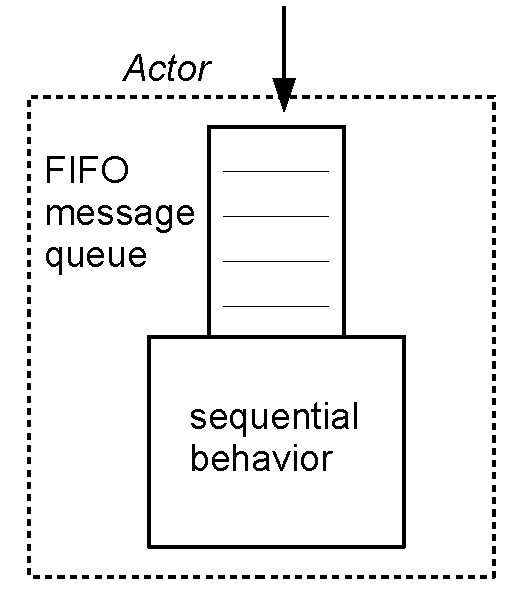
\includegraphics[width=0.4\textwidth]{actor.pdf}
  \caption{Concept of an \textit{Actor} as \\defined by the
          actor model.}
  \label{actor}
  %\vspace{-25mm}
\end{wrapfigure}

The core concepts of the actor model as outlined in \cite{actorsagha}
and \cite{actors2010}
can be summarized as follows. The actor model treats \textit{actors}
(or processes) as its universal primitives of computation.
These actors are autonomous in the sense that each actor's executed
behavior is independent of the concurrent existence of other actors.
However, in order to interact with others, actors can send and receive
messages as illustrated in Fig.\ref{actor}. So each actor consists
of its single threaded behavior and a single input message queue.

The actor can now decide whether or not and how to react to
its incoming messages and can also send messages directly to other
actors. Its behavior itself though is single threaded.
The concurrent nature of an actor based system lies within the
actor model itself because of the actors being executed independent
of each other.

This also means that the only means of communication,
namely message passing, is \textit{asynchronous} by default.
The actor model iself does not define any receipt or acknowledgement mechanism
for messages received by an actors input queue. Any such communication
protocol must be implemented by the actors themselves, e.g. by
programming their behavior to send an acklowdgement to the sender once
a message is processed. This means that, using the plain actor model,
a sender cannot infer whether or not its message was processed
or perceived by its receiver. It cannot even infer whether or not
the message ever reached the receiver.
\newline

This seems ludicrous compared to the implicit safety and messaging
guarantees promised by the \textit{distributed objects} approach
presented in chapter \ref{DistributedObjects} where synchronous
messaging is as \textit{easy} as a local function call. But this
seemingly pessimistic approach to messaging turns out to be
acceptably close that what must be anticipated when dealing with
messaging in highly distributed systems on the data center and cloud
scale.

So again the actor model seems to provide a sweetspot because on
the one hand it encompasses characteristic properties of highly
distributed systems, i.e. virtually no message delivery guarantees,
thereby forcing the developer to deal with these circumstances
\textit{explicitely} in her program structure and application design and on the other
hand provides small, independent and single threaded units of
computation in order to build more abstract and higher level
distributed applications.

\setlength{\intextsep}{10pt}
\setlength{\columnsep}{20pt}

\begin{wrapfigure}{l}{0.5\textwidth}
    \begin{lstlisting}
-module (send_recv).
-compile([export_all]).

serve() ->
  receive
    {Request} ->
      io:format("received request~n"),
      serve()
  end.

run() ->
  Pid = spawn(?MODULE, serve, []),
  Pid ! {Request},
  ok.
    \end{lstlisting}
  \caption{Erlang example of how to spawn an Actor using the \textit{spawn}
          function and how to use the messaging operator \textit{!}}
  \label{erlang-example}
 % \vspace{-20mm}
\end{wrapfigure}

Since Erlang is an actor based language, Fig.\ref{erlang-example}
shows a small example. It spawns an actor executing the
user-defined \textit{serve()} function. Spawning an actor is done
using the built-in \textit{spawn()} function. The serve() function
contains a \textit{receive-loop}, another Erlang built-in indicated
by the \textit{receive} keyword. This loop listens for incoming
messages and tries to match any incoming message to any of the
given patterns. So it can be thought of as the combination of an
implicit event loop and a switch-case statement.

In the case of this example any message that consists of only a single
\texttt{Request} \textit{atom} will be matched to the user-defined
\texttt{Request} \textit{pattern}, triggering
a simple console print and a recursive call to restart the receive
loop. This is important because when the receive loop is entered it
will wait for incoming messages indefinitely unless a timeout is
specified. When a message arrives at the inbox that can be matched
against one of the provided patterns it will be processed as
programmed. When there are multiple messages in the actors inbox
that could be matched against some provided pattern only one
of them is being process and it is up to the actor when to
reenter the receive loop in order to process the remaining messages.
If a message is received that cannot be matched to any pattern, the
message is ignored but kept.
\newline

To address the actor or process created by the call to \textit{spawn()}
a process identifier (PID) is returned by spawn, which is the only
way to attain such an identifier. In order to send messages to this
PID Erlang provides the messaging operator \textit{'!'}.

This shows that message passing is an integral part of the core
language, including its pessimistic delivery guarantees (none), and
specified by the language itself. These semantics are therefor
not loosely defined in some library documentation that could
change any minute but are guaranteed to the programmer,
independent of the language implementation or execution environment.
\newline

Unfortunately there is a down side to this approach. Since the
actor model focusses so heavily on its actors, the result is that
the actual description of the system happens implicitely and
indirectly. It is more like the system \textit{emerges} out of all the
little steps and interactions of its components. To the effect that,
given a running system of maybe a hundred or a thousand actors
\cite{uber}, how would one come to understand what the system is doing
as a whole?

There is no other option than to just pick any actor and start
reading its code. This means one is forced to reverse engineer the
behavior of the entire system from the internal behavior of its parts
which, needless to say, can be quite error prone and introduces
nontrivial cognitive overhead. In other words, there is no way to
take a look at the system from the birds-eye perspective because
most people believe this implies introducing some form of global
state which would be against any of the goals of the actor model
with its asynchronous message passing and independent processes.
\newline

Another problem of the \textit{Actor Model} or any other process
calculus for that matter, is that any actor can possibily communicate
\textit{directly} with any other actor in the entire system at any
given moment in time. This, combined with the fact that almost every
process calculi including the Actor Model is turing-complete,
means that even the simple question whether or not process 1
ever communicates with process 87 becomes undecidable in the general
case. Which makes it almost impossible to predict the consequences
of shutting down a single actor regarding the behavior of the system,
given a large enough system of actors.



\newpage
\ \\
\newpage

\bibliography{0-main}
\bibliographystyle{ieeetr}

% Erzeugen der Selbständigkeitserklärung auf einem neuen Blatt:
\selbstaendigkeitserklaerung{\today}

\end{document}
